\begin{figure}
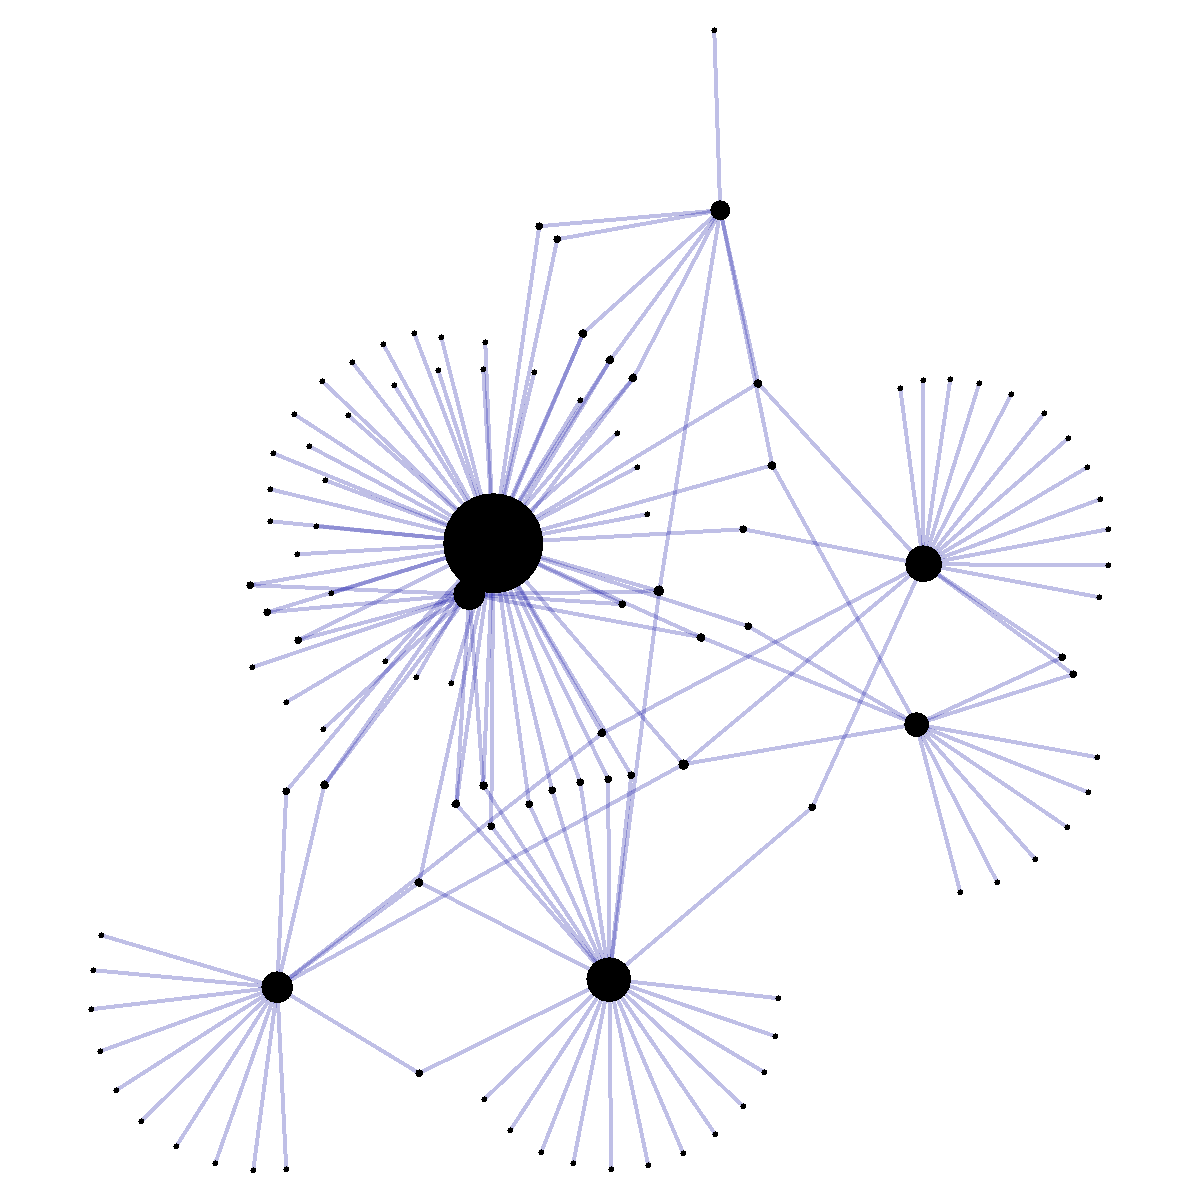
\includegraphics[height=5cm]{simplegraph_by_some_metrics.png}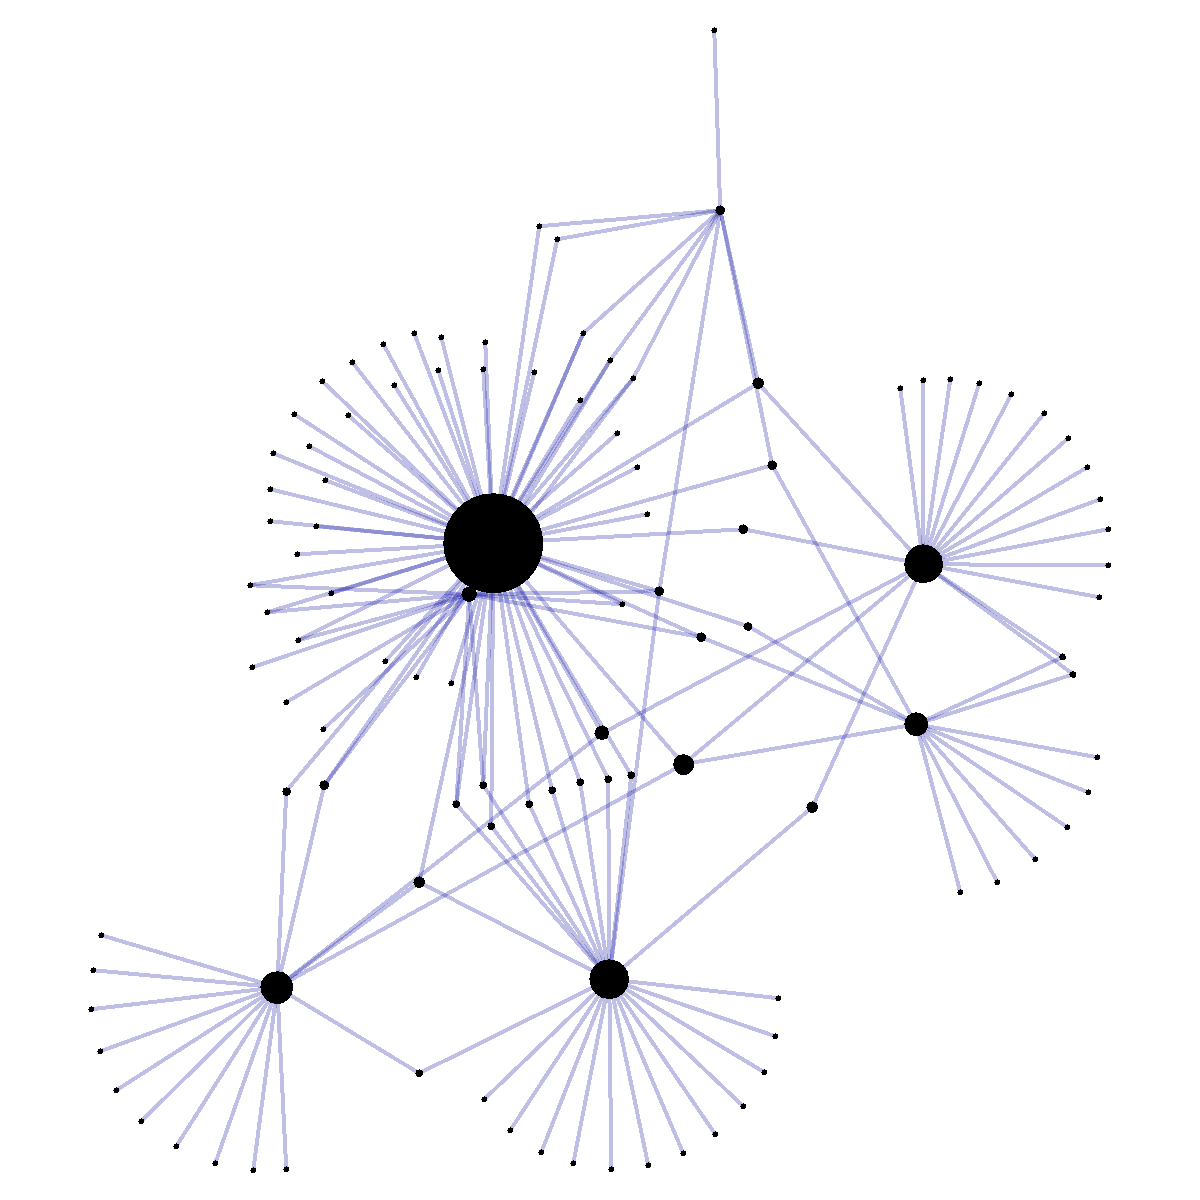
\includegraphics[height=5cm]{simplegraph_by_some_metrics2.png}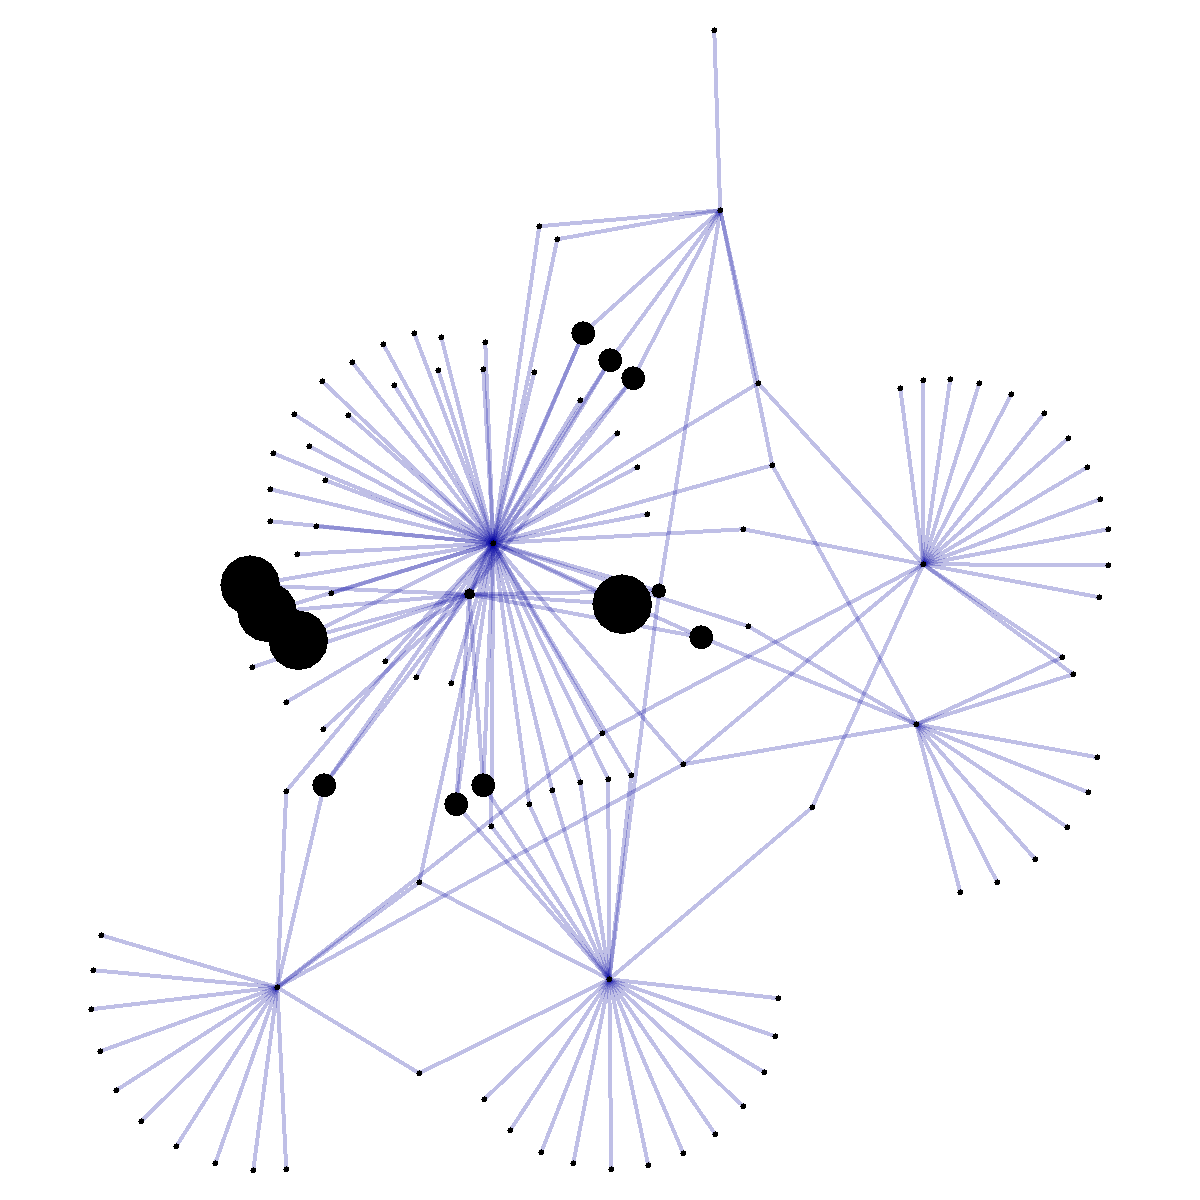
\includegraphics[height=5cm]{simplegraph_by_some_metrics3.png}
\caption{A simple graph with each node's diameter proportional to its \textsl{degree} (1), \textsl{betweenness centrality} (2), and \textsl{local clustering} (3).
In this particular graph, (1) and (2) show similar characteristics (greater value for more ``central'' nodes), whereas local clustering is significantly different.}
\label{fig:simplegraph_by_some_metrics}
\end{figure}
